\section{Przetwarzanie danych}

Lawinowo rosnąca liczba nowych urządzeń podłączanych do sieci
oraz wzrost tempa generowania danych przez nie spodowało,
że konieczne się stało stworzenie nowych metod ich analizy.
Klasyczne metody polegające na tworzeniu coraz większych,
mocniejszych komputerów (\textit{vertical scaling})
mierzących się z problemami analizy danych stawały się nie wystarczające.
Głównie ze względów ekonomicznych.
Takie rozwiązania były bardzo kosztowne w utrzymaniu i szybko stawały się przestarzałe.
Trzeba było szukać pomysłów w innym miejscu.
Zaczęto łączyć mniejsze komputery razem (\textit{horizonal scaling}),
by mogły rozwiązywać większe problemy.
Pojawiły się pierwsze rozwiązania gridowe,
obliczenia chmurowe (\textit{cloud computing})
czy mechanizmy typu \textit{MapReduce}.
Tematykę oraz wszystko co było w okół niej,
związana z masową analizą danych nazwano \textit{Big Data}.

Dane \textit{Big Data} można w skrócie opisać modelem \textit{3V} (Gartner Inc., 2012):
\begin{itemize}
		\item \textbf{Volume} - ilość,
		której nie można przetworzyć z wykorzystaniem standardowych metod i narzędzi.
		\item \textbf{Velocity} - zmienność.
		Dane napływają z różną czestotliwością (natężeniem),
		często w tym samym momencie.
		\item \textbf{Variety} - różnorodność.
		Dane pochodzą pochodzą z wielu źródeł.
		Mogą być lub nie ustrukturyzowane,
		w różnych formatach,
		wymagać wcześniejszego przeprocesowania,
		etc..
\end{itemize}

Obecnie rozwiązania \textit{Big Data} są coraz chętniej wykorzystywane przez firmy.
Począwszy od branży e-commerce,
gdzie są wykorzystywane między innymi do analizy behawioralnej klienta czy prognowania zachowań,
do nawet bezpieczeństwa narodowego
na przykład NSA i program typowania terrorystów.

Główną cechą mechanizmów analizy \textit{Big Data} jest podział zadania
na wiele mniejszych,
niezależnych od siebie podzadań,
które mogą wykonywać się równolegle.
Dzięki dekompozycji zadania na niezależne podzadania,
można niskim kosztem zwiększać wydajność (\textit{throughput})
czy odporność na awarie (\textit{fault-tolerance}) rozwiązania.
Najpopularniejszymi metodami stosowanymi w analizie \textit{Big Data} to
przetwarzanie wsadowe \textit{batch processing}
oraz przetwarzanie strumieniowe \textit{stream processing}.

\subsection{Przetwarznie wsadowe}

Architektura Map Reduce
\begin{figure}[htbp]
\centering
	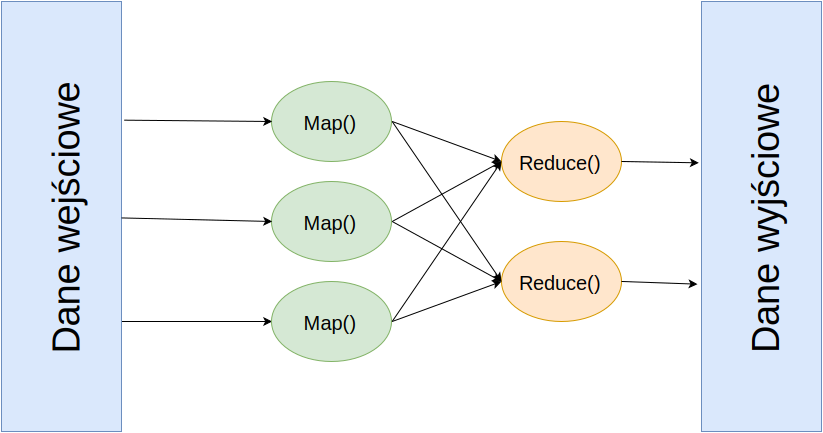
\includegraphics[width=0.8\textwidth]{img/mr}
\end{figure}

\subsection{Przetwarzanie strumieniowe}
